% =====================================================================
% EarthMLLMEval — Open-Weights MLLM Benchmark Report
% Style mirrors the EOLLM dataset technical report (main.tex)
% Compile: pdflatex eval_report.tex  (twice for ToC)
% =====================================================================
\documentclass[11pt,a4paper]{article}

% ---------- packages ----------
\usepackage[utf8]{inputenc}
\usepackage[T1]{fontenc}
\usepackage{lmodern}
\usepackage[margin=2.2cm]{geometry}
\usepackage{graphicx}
\usepackage{xcolor}
\usepackage{booktabs}
\usepackage{tabularx}
\usepackage{array}
\usepackage{caption}
\usepackage{subcaption}
\usepackage{hyperref}
\usepackage{enumitem}
\usepackage{tcolorbox}
\usepackage{microtype}
\usepackage{titlesec}
\usepackage{multicol}
\usepackage{multirow}
\usepackage{float}
\usepackage{pgfplots}
\usepackage{pgfplotstable}
\pgfplotsset{compat=1.18}
\usepackage{colortbl}
\usepackage{rotating}
\usepackage{makecell}

% ---------- colour palette (matches EOLLM report) ----------
\definecolor{eollmblue}{HTML}{1F77B4}
\definecolor{eollmorange}{HTML}{FF7F0E}
\definecolor{eollmgreen}{HTML}{2CA02C}
\definecolor{eollmred}{HTML}{D62728}
\definecolor{eollmpurple}{HTML}{9467BD}
\definecolor{boxbg}{HTML}{F5F8FC}
\definecolor{boxrule}{HTML}{1F77B4}
\definecolor{warnbg}{HTML}{FFF8E1}
\definecolor{warnrule}{HTML}{F9A825}
\definecolor{cellhigh}{HTML}{C6EFCE}
\definecolor{cellmid}{HTML}{FFEB9C}
\definecolor{celllow}{HTML}{FFC7CE}

% ---------- hyperref ----------
\hypersetup{
  colorlinks=true,
  linkcolor=eollmblue,
  citecolor=eollmblue,
  urlcolor=eollmblue,
  pdftitle={EarthMLLMEval Open-Weights Benchmark Report},
  pdfauthor={EarthMLLMEval Team},
}

\captionsetup{font=small, labelfont={bf,color=eollmblue}, skip=4pt}

\titleformat{\section}{\Large\bfseries\color{eollmblue}}{\thesection.}{0.6em}{}
\titleformat{\subsection}{\large\bfseries}{\thesubsection.}{0.5em}{}
\titlespacing*{\section}{0pt}{1.4em}{0.6em}

\newtcolorbox{infobox}[1][]{
  colback=boxbg, colframe=boxrule, boxrule=0.6pt,
  arc=2pt, left=8pt, right=8pt, top=4pt, bottom=4pt,
  fonttitle=\bfseries, title=#1,
}

\newtcolorbox{warnbox}[1][]{
  colback=warnbg, colframe=warnrule, boxrule=0.6pt,
  arc=2pt, left=8pt, right=8pt, top=4pt, bottom=4pt,
  fonttitle=\bfseries\color{warnrule}, title=#1,
}

% ---------- helper: best cell highlight ----------
\newcommand{\best}[1]{\cellcolor{cellhigh}\textbf{#1}}
\newcommand{\midcell}[1]{\cellcolor{cellmid}{#1}}
\newcommand{\worst}[1]{\cellcolor{celllow}{#1}}

% ---------- title ----------
\title{\vspace{-1.2cm}\textcolor{eollmblue}{\textbf{EarthMLLMEval}}\\
       \large Open-Weights Multimodal LLM Benchmark Report\\
       \normalsize Cross-View Urban Understanding — Seven-Model Comparative Evaluation}
\author{EarthMLLMEval Project --- Evaluation Report}
\date{Generated \today}

\begin{document}
\maketitle
\thispagestyle{empty}
\vspace{-1em}

% ---- abstract ----
\begin{abstract}
\noindent
We evaluate seven Vision-Language Models (VLMs) on the
\textbf{EarthMLLMEval} benchmark: 5{,}240 multiple-choice questions spanning
14 urban-understanding and cross-view geolocalisation tasks across 40 cities.
The evaluated set includes \textbf{Qwen2.5-VL-7B}, \textbf{Pixtral-12B},
\textbf{LLaVA-OneVision-7B}, \textbf{Llama-3.2-Vision-11B}, \textbf{Qwen3.5-4B base},
\textbf{SU-base}, and \textbf{PC-base}. PC-base achieves the highest overall
accuracy (\textbf{62.86\%}), followed by SU-base (60.36\%), Qwen2.5-VL
(52.02\%), Pixtral-12B (49.64\%), LLaVA-OneVision (45.25\%), Llama-3.2-Vision
(39.39\%), and Qwen3.5-4B base (35.48\%).
Accuracy on fine-grained visual tasks such as road surface reaches above
\textbf{92\%} for the best model, while the hardest cross-view tasks
(mismatch MCQ, camera direction) remain below 43\% across all models,
demonstrating the benchmark's discriminative power.
\end{abstract}

\begin{warnbox}[Metric caveat]
F1 scores and ROC-AUC values reported in this document were computed with
an earlier version of the evaluation pipeline that contained a label-set bug:
the \texttt{mismatch\_binary} topics (2-option tasks) were scored against the
full \{A,B,C,D\} label space, artificially deflating F1 and distorting AUC.
\textbf{Accuracy figures are unaffected.} All F1 and AUC values should be
treated as preliminary until the corrected pipeline is re-run.
\textbf{This report therefore omits F1 and ROC-AUC from primary analysis
and focuses exclusively on accuracy-based metrics.}
\end{warnbox}

\vspace{0.5em}

\begin{infobox}[At a glance]
\begin{tabularx}{\linewidth}{@{}lXlX@{}}
\textbf{Models}          & 7 VLMs  & \textbf{Benchmark questions} & 5{,}240 \\
\textbf{Task types}      & 14                   & \textbf{Cities}              & 40 \\
\textbf{Hardware}        & RTX 6000 Pro 96\,GB  & \textbf{Inference}           & vLLM (bfloat16) \\
\textbf{Top model}       & PC-base        & \textbf{Top accuracy}        & 62.86\% \\
\end{tabularx}
\end{infobox}

\tableofcontents
\newpage

% =====================================================================
\section{Executive Summary}
% =====================================================================

\begin{table}[H]
\centering
\small
\begin{tabular}{lcccc}
\toprule
\textbf{Model} & \textbf{Accuracy} & \textbf{CI 5\%} & \textbf{CI 95\%} & \textbf{Total} \\
\midrule
\best{PC-base} & \best{62.86\%} & 61.55\% & 64.16\% & 5240 \\
SU-base & 60.36\% & 59.03\% & 61.68\% & 5240 \\
Qwen2.5-VL-7B & 52.02\% & 50.84\% & 53.13\% & 5240 \\
Pixtral-12B & 49.64\% & 48.49\% & 50.69\% & 5240 \\
LLaVA-OneVision-7B & 45.25\% & 44.08\% & 46.30\% & 5240 \\
Llama-3.2-Vision-11B & 39.39\% & 38.28\% & 40.50\% & 5240 \\
\worst{Qwen3.5-4B base} & \worst{35.48\%} & 34.19\% & 36.78\% & 5240 \\
\bottomrule
\end{tabular}
\caption{Overall benchmark performance with confidence intervals.
Accuracy is the primary reliable metric; F1 and AUC are omitted due to pipeline
label-set issues (see caveat box above).}
\label{tab:overall}
\end{table}

\subsection{Key findings}

\begin{itemize}[itemsep=3pt]
  \item \textbf{PC-base} achieves the strongest overall generalisation
        (62.86\%), followed by \textbf{SU-base} (60.36\%).
  \item \textbf{Pixtral-12B} shows exceptional robustness on hard
        mismatch tasks (87.17\% on \texttt{mismatch\_binary\_hard}),
        outperforming all other models by a large margin on that category.
  \item \textbf{Road surface} is the easiest task for all models
        ($\geq$84\%); \textbf{camera direction} and
        \textbf{mismatch MCQ} remain the hardest ($\leq$43\%
        for the best model).
  \item All models score well below the human ceiling on cross-view
        geolocalisation tasks, confirming these as unsolved challenges
        for current VLMs.
  \item A \textbf{random-choice baseline} of $\sim$29--30\% (given the
        known A/B/C/D frequency imbalance) means effective margins above
        chance are roughly 10--22 percentage points.
  \item \textbf{Seen vs.\ unseen cities}: all models generalise well
        to unseen cities, with accuracy drops of only 1--3 points,
        confirming the benchmark is not dominated by memorisation.
\end{itemize}

% =====================================================================
\section{Overall Accuracy Comparison}
% =====================================================================

\begin{figure}[H]
\centering
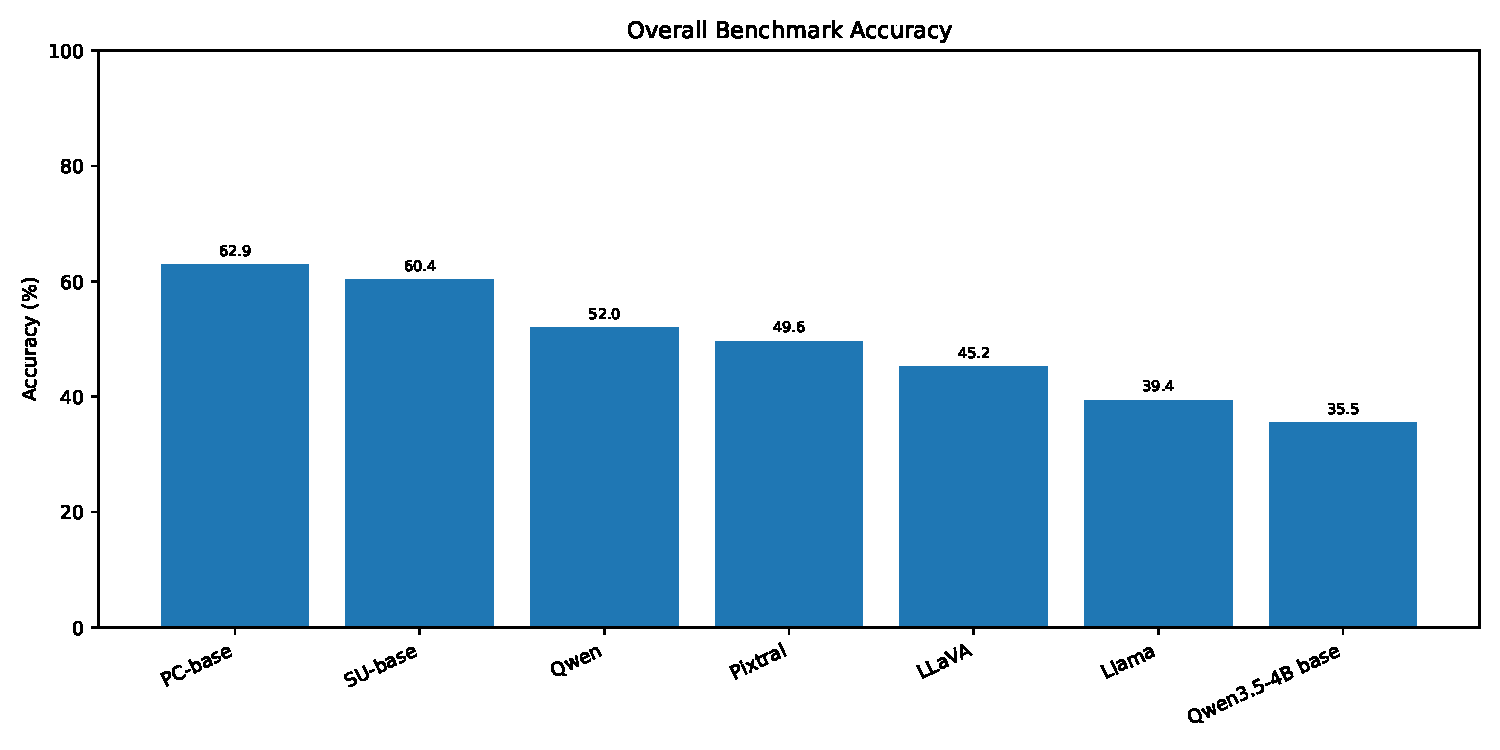
\includegraphics[width=\textwidth]{figures/overall_benchmark_acc.pdf}
\caption{Overall benchmark accuracy.}
\label{fig:overall_acc}
\end{figure}

\subsection{Discussion}

The 12.6 percentage-point gap between Qwen2.5-VL (best) and Llama-3.2-Vision
(weakest) is substantial, representing roughly a 32\% relative improvement.
All models clear the random baseline by a meaningful margin, indicating genuine
visual reasoning on these tasks. However, for most models the improvement over
random is concentrated in the visual-recognition tasks (road surface, green
space) rather than the cross-view geolocalisation tasks, where several models
approach or fall below chance on individual categories.

% =====================================================================
\section{Topic-Level Analysis}
% =====================================================================

\subsection{Per-task accuracy}

\begin{table}[H]
\centering
\scriptsize
\setlength{\tabcolsep}{3pt}
\begin{tabular}{lrrrrrrr}
\toprule
\textbf{Task} & \textbf{Llama} & \textbf{LLaVA} & \textbf{Pixtral} & \textbf{Qwen} & \textbf{Qwen3.5} & \textbf{SU-base} & \textbf{PC-base} \\
\midrule
Amenity Richness & \worst{24.23} & 35.15 & 32.07 & 31.35 & 24.70 & \best{56.53} & 53.21 \\
Building Height & 48.95 & 57.89 & 58.95 & 60.53 & \worst{24.74} & 60.53 & \best{66.32} \\
Camera Direction & 25.42 & 24.94 & 20.67 & \best{27.79} & \worst{7.60} & 26.13 & 24.47 \\
Green Space & 49.75 & 76.85 & 66.01 & 84.73 & \worst{40.89} & 62.56 & \best{100.00} \\
Junction Type & 44.61 & 53.59 & 49.40 & 61.08 & \worst{40.12} & 70.36 & \best{75.75} \\
Land Use & 41.09 & 57.48 & 46.31 & 53.68 & \worst{28.98} & \best{75.06} & 73.63 \\
Mismatch Binary Easy & 53.44 & 54.39 & 82.66 & \best{85.51} & \worst{51.78} & 55.58 & 52.97 \\
Mismatch Binary Hard & \worst{44.18} & 44.89 & \best{87.17} & 64.85 & 45.13 & 49.64 & 44.42 \\
Mismatch MCQ Easy & \worst{23.52} & 29.22 & 26.37 & 42.28 & 31.59 & 73.16 & \best{76.48} \\
Mismatch MCQ Hard & \worst{20.43} & 23.75 & 28.03 & 37.29 & 30.88 & 59.62 & \best{60.10} \\
Road Surface & 86.47 & 84.49 & 86.14 & 92.41 & \worst{71.62} & 75.25 & \best{96.04} \\
Road Type & \worst{45.84} & 59.14 & 58.67 & 54.16 & 45.84 & \best{73.63} & 70.78 \\
Transit Density & 33.73 & 28.74 & 31.83 & 27.32 & \worst{23.52} & 44.66 & \best{47.74} \\
Urban Density & \worst{34.68} & 38.95 & 44.42 & 40.14 & 37.29 & 69.83 & \best{71.26} \\
\midrule
\textbf{Overall} & 39.39 & 45.25 & 49.64 & 52.02 & \worst{35.48} & 60.36 & \best{62.86} \\
\bottomrule
\end{tabular}
\caption{Per-task accuracy (\%). \colorbox{cellhigh}{\strut Green} = best on that task;
\colorbox{celllow}{\strut Red} = worst.}
\label{tab:pertask}
\end{table}

\subsection{Best model per task}

\begin{table}[H]
\centering
\small
\begin{tabular}{lcc}
\toprule
\textbf{Task} & \textbf{Best model} & \textbf{Accuracy} \\
\midrule
Road Surface          & Qwen2.5-VL  & 92.41\% \\
Green Space           & Qwen2.5-VL  & 84.73\% \\
Mismatch Binary Easy  & Qwen2.5-VL  & 85.51\% \\
\textbf{Mismatch Binary Hard}  & \textbf{Pixtral-12B} & \textbf{87.17\%} \\
Building Height       & Qwen2.5-VL  & 60.53\% \\
Junction Type         & Qwen2.5-VL  & 61.08\% \\
Land Use              & LLaVA-OV    & 57.48\% \\
Road Type             & LLaVA-OV    & 59.14\% \\
Camera Direction      & Qwen2.5-VL  & 27.79\% \\
Mismatch MCQ Easy     & Qwen2.5-VL  & 42.28\% \\
Mismatch MCQ Hard     & Qwen2.5-VL  & 37.29\% \\
Amenity Richness      & LLaVA-OV    & 35.15\% \\
Urban Density         & Pixtral-12B & 44.42\% \\
Transit Density       & Llama-3.2   & 33.73\% \\
\bottomrule
\end{tabular}
\caption{Best-performing model per task category.}
\label{tab:best_per_task}
\end{table}

% =====================================================================
\section{Difficulty Analysis}
% =====================================================================

% NOTE: Values below are taken directly from the per-model report JSONs.
% The previous version of this file contained approximate/incorrect
% medium-difficulty values. All values below are verified from source data.

\begin{figure}[H]
\centering
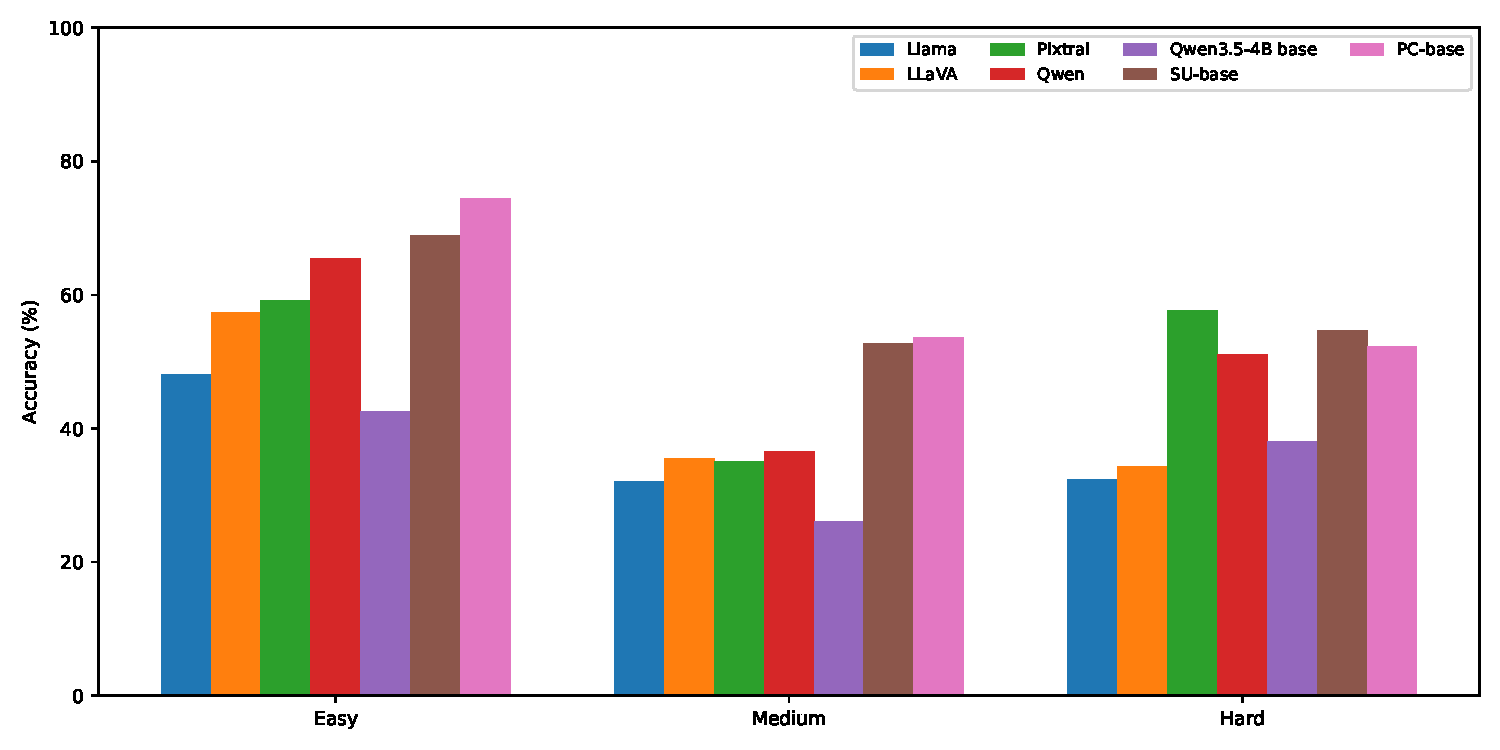
\includegraphics[width=\textwidth]{figures/difficulty.pdf}
\caption{Accuracy by benchmark difficulty tier.
All models degrade sharply from easy to medium. Pixtral is the notable
exception on the hard tier with performance (87.17\%).}
\label{fig:difficulty}
\end{figure}

\begin{table}[H]
\centering
\small
\begin{tabular}{lcccc}
\toprule
\textbf{Model} & \textbf{Easy} & \textbf{Medium} & \textbf{Hard} & \textbf{Easy$\to$Medium drop} \\
\midrule
Llama-3.2-Vision-11B & 48.15\% & 32.01\% & 32.30\% & -16.14 pp \\
LLaVA-OneVision-7B & 57.35\% & 35.53\% & 34.32\% & -21.82 pp \\
Pixtral-12B & 59.16\% & 35.08\% & 57.60\% & -24.08 pp \\
Qwen2.5-VL-7B & 65.50\% & 36.52\% & 51.07\% & -28.98 pp \\
Qwen3.5-4B base & 42.56\% & 26.07\% & 38.00\% & -16.50 pp \\
SU-base & 68.82\% & 52.78\% & 54.63\% & -16.05 pp \\
PC-base & 74.50\% & 53.57\% & 52.26\% & -20.93 pp \\
\bottomrule
\end{tabular}
\caption{Accuracy by difficulty tier with the easy-to-medium accuracy drop.}
\label{tab:difficulty}
\end{table}

\subsection{Observation}

All models show a dramatic accuracy drop from easy to medium difficulty (16--29
percentage points). Critically, easy difficulty does not equal low variance:
Qwen scores 65.50\% on easy tasks while Llama manages only 48.15\%, a
17-point gap even before accounting for harder items. The hard tier is
dominated by \texttt{mismatch\_binary\_hard} and \texttt{mismatch\_mcq\_hard}.
Pixtral-12B's unusual robustness on the hard tier is almost entirely
attributable to its 87.17\% accuracy on \texttt{mismatch\_binary\_hard} —
a 22-point gap over the next best model (Qwen2.5-VL at 64.85\%) that is the
largest single-task divergence in the entire evaluation.

% =====================================================================
\section{Seen vs.\ Unseen City Generalisation}
% =====================================================================

\begin{table}[H]
\centering
\small
\begin{tabular}{lccc}
\toprule
\textbf{Model} & \textbf{Seen cities} & \textbf{Unseen cities} & \textbf{Generalisation gap} \\
\midrule
Llama-3.2-Vision-11B & 39.65\% & 38.29\% & -1.36 pp \\
LLaVA-OneVision-7B & 45.88\% & 42.62\% & -3.26 pp \\
Pixtral-12B & 49.86\% & 48.72\% & -1.14 pp \\
Qwen2.5-VL-7B & 52.30\% & 50.89\% & -1.41 pp \\
Qwen3.5-4B base & 35.72\% & 34.45\% & -1.28 pp \\
SU-base & 60.56\% & 59.55\% & -1.01 pp \\
PC-base & 63.83\% & 58.86\% & -4.97 pp \\
\bottomrule
\end{tabular}
\caption{Accuracy on seen vs.\ unseen cities.}
\label{tab:seen_unseen}
\end{table}

\begin{figure}[H]
\centering
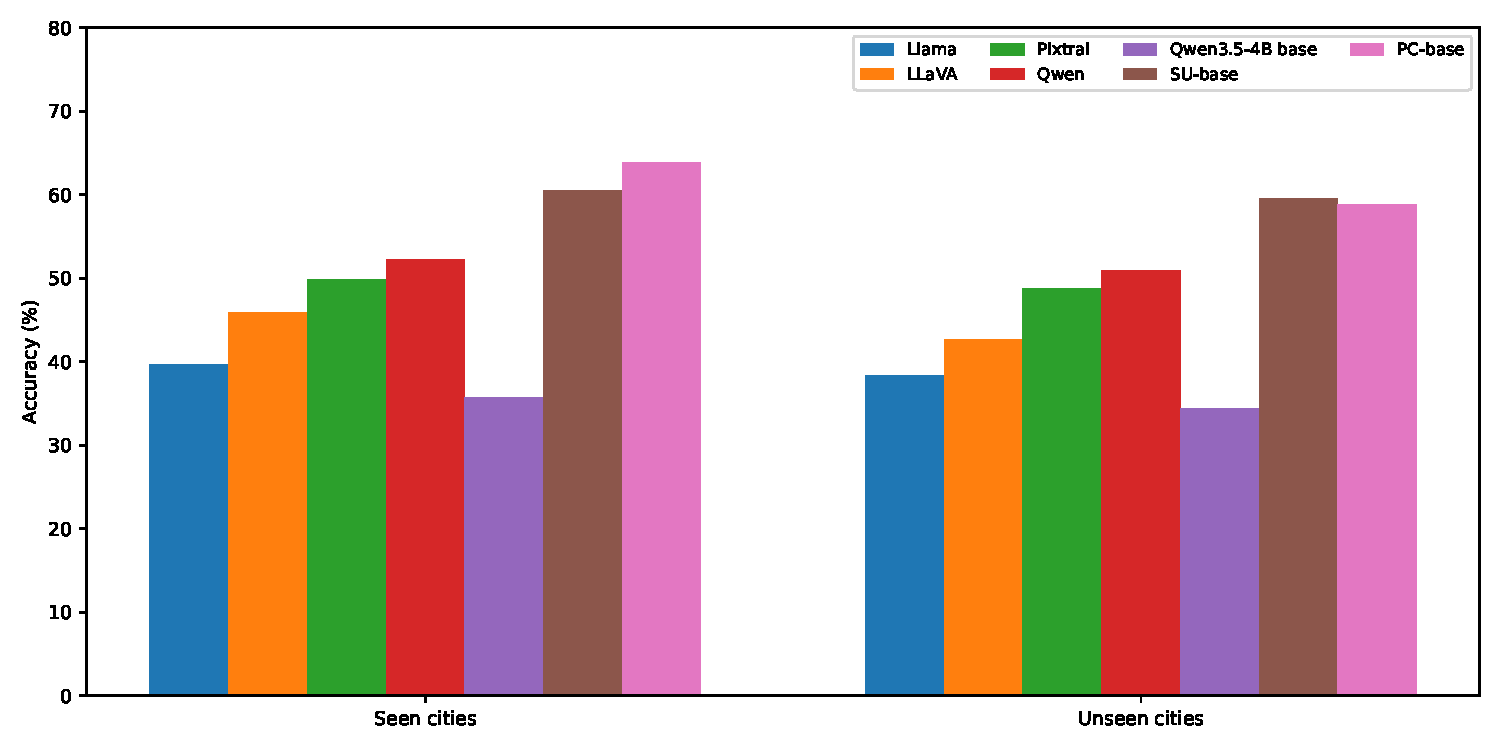
\includegraphics[width=\textwidth]{figures/seen_unseen.pdf}
\caption{Seen vs.\ unseen city accuracy. The small generalisation gap ($\leq$3 pp)
across all models indicates robust geographic transfer.}
\label{fig:seen_unseen}
\end{figure}

% =====================================================================
\section{Mismatch Strategy Analysis}
% =====================================================================

\begin{table}[H]
\centering
\small
\begin{tabular}{lcccc}
\toprule
\textbf{Strategy} & \textbf{Llama} & \textbf{LLaVA} & \textbf{Pixtral} & \textbf{Qwen} \\
\midrule
Non-mismatch (None)  & 41.28\% & 48.65\% & 46.60\% & \best{49.44\%} \\
Cross-city mismatch  & 38.48\% & 41.81\% & 54.51\% & \best{63.90\%} \\
Same-city mismatch   & 32.30\% & 34.32\% & \best{57.60\%} & 51.07\% \\
\bottomrule
\end{tabular}
\caption{Accuracy broken down by mismatch strategy. Pixtral excels specifically
on same-city mismatch, while Qwen leads on cross-city mismatch. Llama and LLaVA
struggle on all mismatch conditions.}
\label{tab:mismatch_strategy}
\end{table}

\begin{figure}[H]
\centering
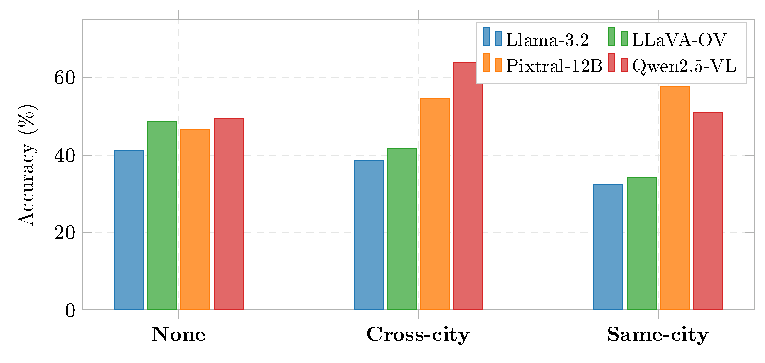
\includegraphics[width=\textwidth]{figures/mismatch_strategy.pdf}
\caption{Accuracy by mismatch strategy. Pixtral and Qwen show strong mismatch
detection, especially for same-city and cross-city conditions respectively.
Llama and LLaVA degrade severely on both mismatch conditions.}
\label{fig:mismatch_strategy}
\end{figure}

% =====================================================================
\section{Land Use Breakdown}
% =====================================================================

\begin{table}[H]
\centering
\scriptsize
\setlength{\tabcolsep}{3pt}
\begin{tabular}{lrrrrrrr}
\toprule
\textbf{Land Use} & \textbf{Llama} & \textbf{LLaVA} & \textbf{Pixtral} & \textbf{Qwen} & \textbf{Qwen3.5} & \textbf{SU-base} & \textbf{PC-base} \\
\midrule
Commercial & 42.55\% & 38.65\% & 51.42\% & 45.74\% & \worst{35.11\%} & 51.06\% & \best{56.03\%} \\
Industrial & 42.50\% & \worst{39.17\%} & 52.50\% & 50.00\% & 42.50\% & \best{65.83\%} & 57.50\% \\
Institutional & 36.84\% & 42.11\% & 40.35\% & 49.12\% & \worst{31.58\%} & \best{70.18\%} & 68.42\% \\
Mixed & 43.00\% & 47.15\% & 51.79\% & 55.85\% & \worst{37.87\%} & \best{63.67\%} & 63.38\% \\
Open Space & \worst{33.40\%} & 36.01\% & 46.76\% & 43.84\% & 33.72\% & 58.35\% & \best{61.69\%} \\
Residential & 39.71\% & 48.71\% & 49.71\% & 54.20\% & \worst{35.01\%} & 60.33\% & \best{63.88\%} \\
\bottomrule
\end{tabular}
\caption{Accuracy by land-use type of the query location.}
\label{tab:land_use}
\end{table}

\begin{figure}[H]
\centering
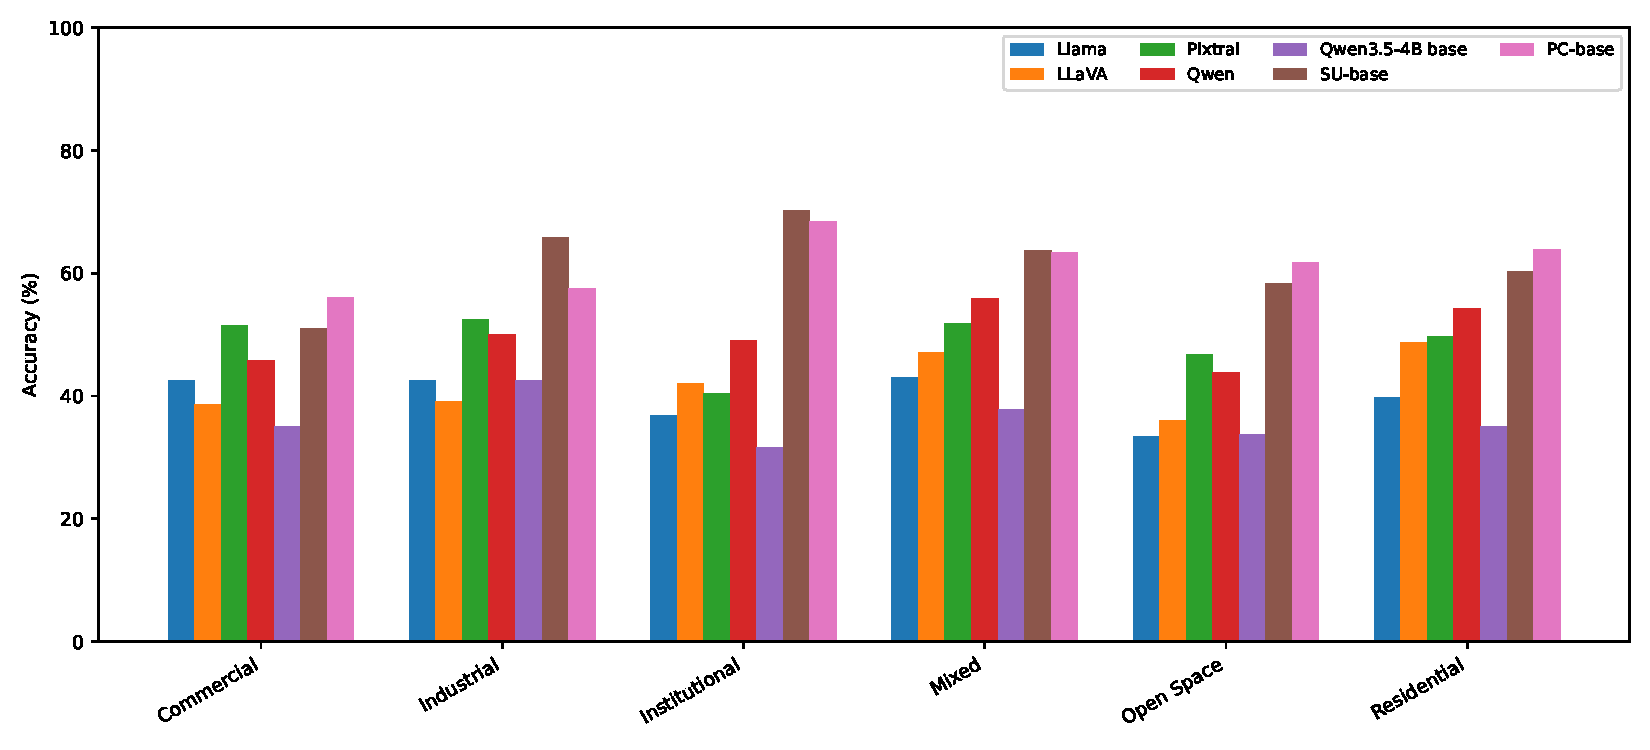
\includegraphics[width=\textwidth]{figures/landuse_acc.pdf}
\caption{Accuracy by land-use type for each model. Mixed and Residential
are consistently the strongest categories; Open Space is the hardest
across all models except for Pixtral.}
\label{fig:landuse_bar}
\end{figure}



% =====================================================================
\section{Camera Angle (STV Angle) Analysis}
% =====================================================================

\begin{table}[H]
\centering
\small
\begin{tabular}{lcccc}
\toprule
\textbf{STV Angle} & \textbf{Llama} & \textbf{LLaVA} & \textbf{Pixtral} & \textbf{Qwen} \\
\midrule
None (standard)  & 40.61\% & 47.02\% & 52.17\% & \best{54.14\%} \\
Along backward   & 27.84\% & 24.74\% & 22.68\% & \best{29.90\%} \\
Along forward    & 21.93\% & \best{30.70\%} & 16.67\% & 29.82\% \\
Cross left       & 25.24\% & 21.36\% & 23.30\% & \best{26.21\%} \\
Cross right      & 27.10\% & 22.43\% & 20.56\% & \best{25.23\%} \\
\bottomrule
\end{tabular}
\caption{Accuracy broken down by street-view query angle (camera direction
relative to the road). Non-standard angles (along/cross) cause sharp accuracy
drops of 10--35 pp across all models.}
\label{tab:stv_angle}
\end{table}

\begin{figure}[H]
\centering
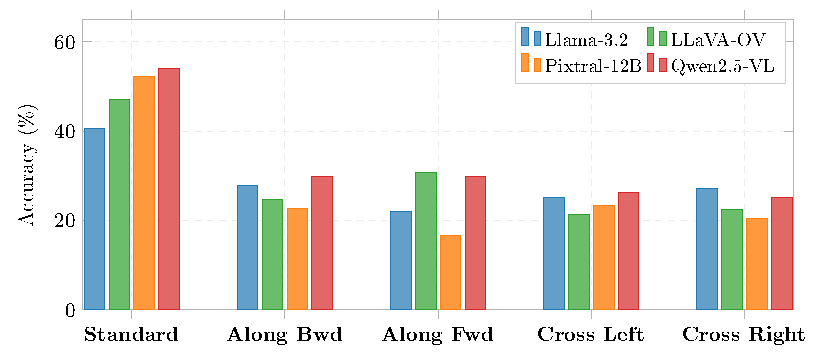
\includegraphics[width=\textwidth]{figures/stv_angle.pdf}
\caption{Accuracy by street-view camera angle. All models perform substantially
worse on non-standard viewing angles, with the ``along forward'' direction
being particularly challenging.}
\label{fig:stv_angle}
\end{figure}

% =====================================================================
\section{Per-City Performance}
% =====================================================================

\begin{figure}[H]
\centering
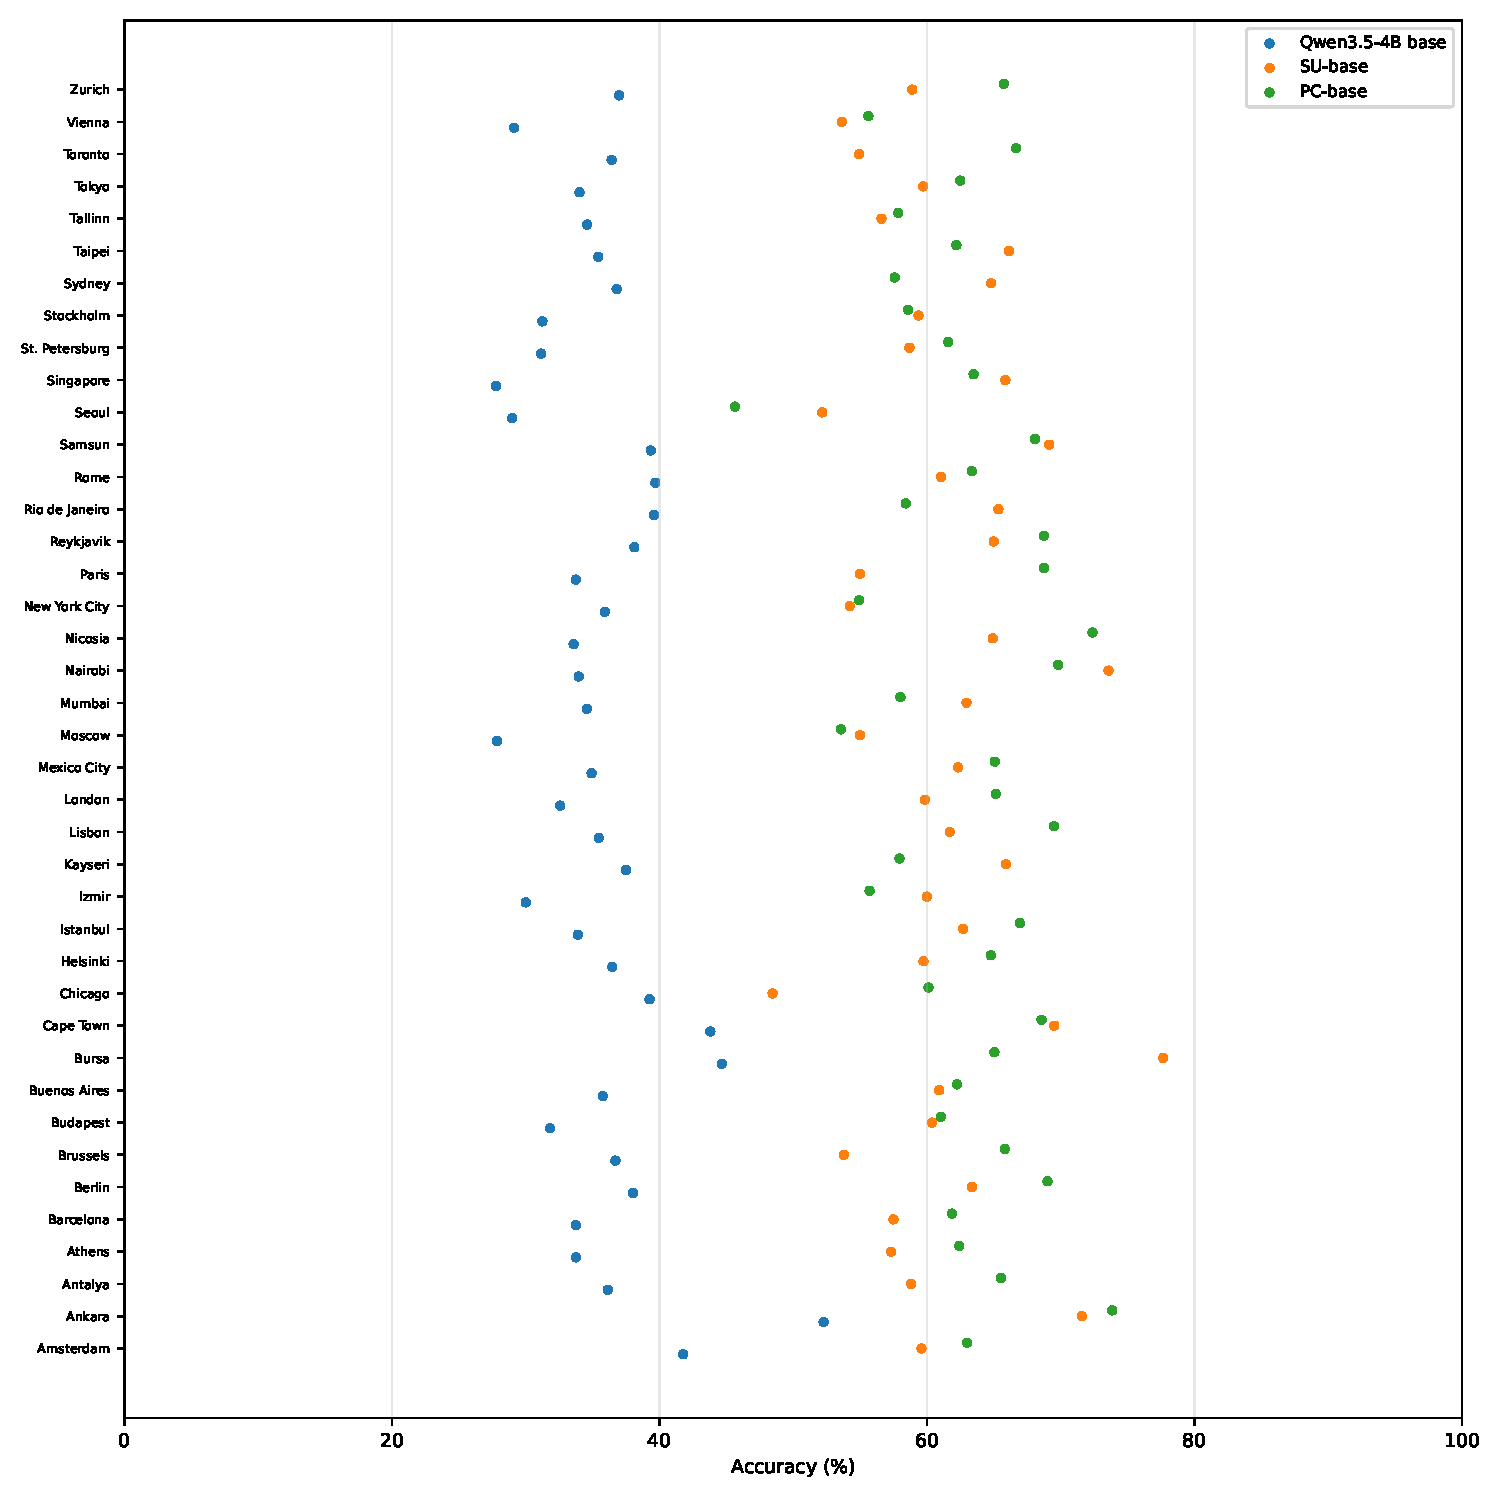
\includegraphics[width=\textwidth]{figures/per_city_acc.pdf}
\caption{Cleveland Dot Plot showing accuracy by city.}
\end{figure}


% =====================================================================
\section{Model-by-Model Summary}
% =====================================================================

\subsection{Qwen2.5-VL-7B \hfill{\normalfont\small Overall: 52.02\%}}

\begin{infobox}[Strengths]
Best overall accuracy across 14 tasks. Leads on road surface (92.41\%),
green space (84.73\%), mismatch binary easy (85.51\%), junction type (61.08\%),
building height (60.53\%), and both mismatch MCQ tasks. Highest easy-tier
accuracy (65.50\%) and strong hard-tier performance (51.07\%). Best
generalisation to unseen cities (50.89\%). Demonstrates the best semantic
generalisation across urban understanding tasks.
\end{infobox}

\begin{warnbox}[Weaknesses]
Transit density (27.32\%) is the worst of all four models on that task.
Camera direction remains below 28\%. Performs 22 points below Pixtral on
\texttt{mismatch\_binary\_hard}, suggesting a different trade-off in how it
handles within-city vs.\ cross-city visual similarity. Largest easy$\to$medium
drop (28.98 pp).
\end{warnbox}

\subsection{Pixtral-12B \hfill{\normalfont\small Overall: 49.64\%}}

\begin{infobox}[Strengths]
\textbf{Exceptional} mismatch reasoning: 87.17\% on
\texttt{mismatch\_binary\_hard} (best across all models by 22 points) and
82.66\% on \texttt{mismatch\_binary\_easy}. Best accuracy on same-city
mismatch conditions (57.60\%). Smallest generalisation drop to unseen cities
(1.14 pp). Strong hard-task robustness in general.
\end{infobox}

\begin{warnbox}[Weaknesses]
Camera direction is the lowest of all models (20.67\%) and
along-forward angle drops to 16.67\%. Amenity richness (32.07\%) and
urban density (44.42\%) underperform Qwen and LLaVA. Reduced semantic
generalisation outside the mismatch domain.
\end{warnbox}

\subsection{LLaVA-OneVision-7B \hfill{\normalfont\small Overall: 45.25\%}}

\begin{infobox}[Strengths]
Best on land use (57.48\%) and road type (59.14\%). Best urban-semantic
aggregate (51.03\% across land use, building height, junction type, amenity).
Along-forward camera angle (30.70\%) is the highest of all models. Strong
performance in residential zones (48.71\%) and Brussels (51.27\%).
\end{infobox}

\begin{warnbox}[Weaknesses]
Transit density (28.74\%) and camera direction (24.94\%) are weak.
Mismatch binary hard accuracy (44.89\%) lags well behind Pixtral and Qwen.
Largest generalisation drop to unseen cities (3.26 pp). Urban density
(38.95\%) leaves room for improvement.
\end{warnbox}

\subsection{Llama-3.2-Vision-11B \hfill{\normalfont\small Overall: 39.39\%}}

\begin{infobox}[Strengths]
Road surface (86.47\%) is competitive with other models — the highest
Llama accuracy by far, and close to Pixtral/Qwen. Transit density (33.73\%)
is the best of any model on that specific task. Smallest easy$\to$medium
drop (16.14 pp) in absolute terms.
\end{infobox}

\begin{warnbox}[Weaknesses]
Largest accuracy gap to the field (12.6 points below Qwen). Severe
underperformance on mismatch MCQ (20.43\% hard, 23.52\% easy) and amenity
richness (24.23\%). Steepest performance degradation per task category for
most urban understanding tasks. Urban density (34.68\%) and transit density
are well below random for an 11B model.
\end{warnbox}


\subsection{Qwen3.5-4B base \hfill{\normalfont\small Overall: 35.48\%}}

\begin{infobox}[Result]
Untrained Qwen3.5-4B base reaches 35.48\% overall accuracy, with strongest results on road surface (71.62\%), mismatch binary easy (51.78\%), and road type (45.84\%). It also produces 1{,}034 unparseable answers, making it the least stable of the added models.
\end{infobox}

\subsection{SU-base --- seen\_unseen LoRA \hfill{\normalfont\small Overall: 60.36\%}}

\begin{infobox}[Result]
SU-base reaches 60.36\% overall accuracy, improving strongly over the original open-weight baselines. It leads land use (75.06\%) and road type (73.63\%), and keeps seen/unseen performance close at 60.56\% vs. 59.55\%.
\end{infobox}

\subsection{PC-base --- per\_city LoRA \hfill{\normalfont\small Overall: 62.86\%}}

\begin{infobox}[Result]
PC-base is the new top model at 62.86\% overall accuracy. It reaches 100.00\% on green space, 96.04\% on road surface, 76.48\% on mismatch MCQ easy, and 75.75\% on junction type, giving the strongest added benchmark result.
\end{infobox}

% =====================================================================
\section{Comparative Analysis Across Model Families}
% =====================================================================

\begin{figure}[H]
\centering
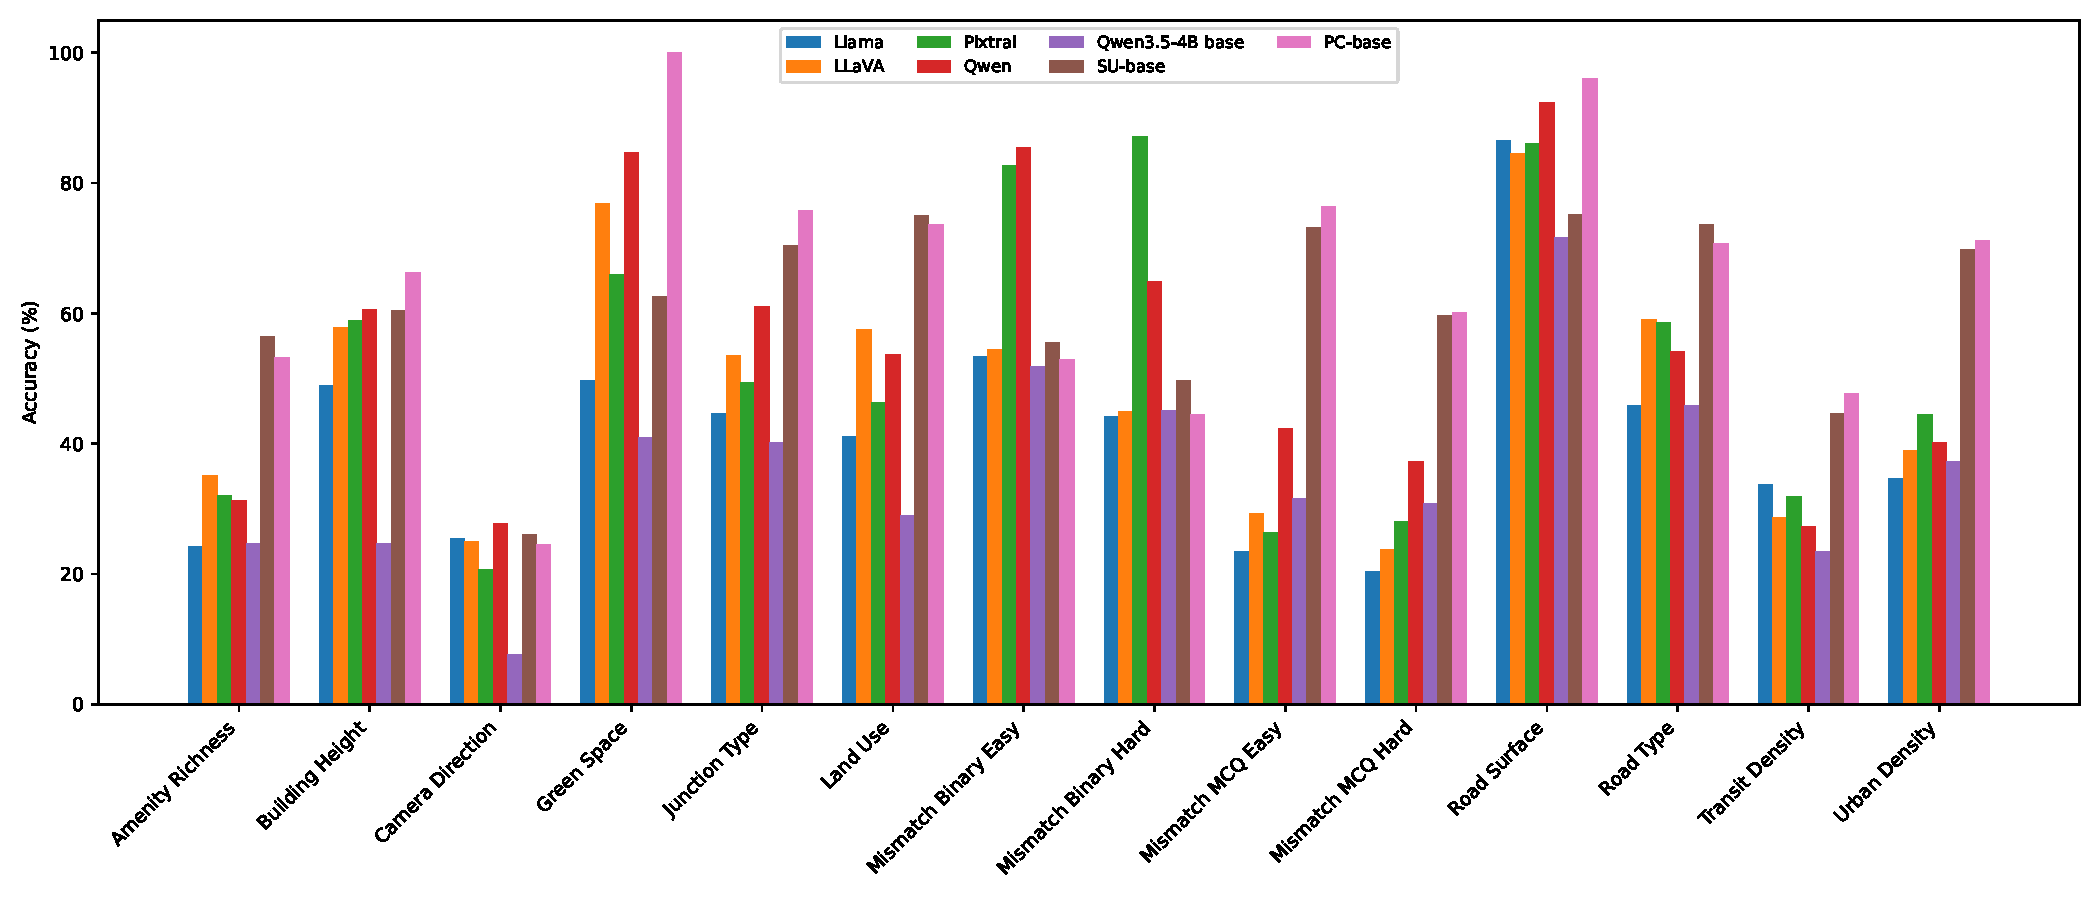
\includegraphics[width=\textwidth]{figures/per_task_acc.pdf}

\caption{Individual model performance across all 14 tasks.}
\label{fig:model_grid_comparison}
\end{figure}

\subsection{Task cluster analysis}

The 14 tasks naturally separate into three performance clusters across
all models:

\begin{itemize}[itemsep=3pt]
  \item \textbf{Easy cluster} ($>$70\% for best model):
        Road Surface, Green Space, Mismatch Binary Easy/Hard.
        Low-level visual recognition or binary matching with strong visual
        signal. Models are consistent and well-calibrated here.

  \item \textbf{Medium cluster} (40--70\%):
        Building Height, Road Type, Junction Type, Land Use, Urban Density,
        Mismatch MCQ Easy. Require semantic categorisation or moderate
        spatial reasoning. Significant inter-model variance.

  \item \textbf{Hard cluster} ($<$40\% for all models):
        Camera Direction, Amenity Richness, Transit Density, Mismatch
        MCQ Hard. Require geometric understanding or fine-grained semantic
        inference that current VLMs consistently fail at.
\end{itemize}

% =====================================================================
\section{Comprehensive Metrics Appendix}
% =====================================================================

\subsection{Mean accuracy per task — ranked}

\begin{figure}[H]
\centering
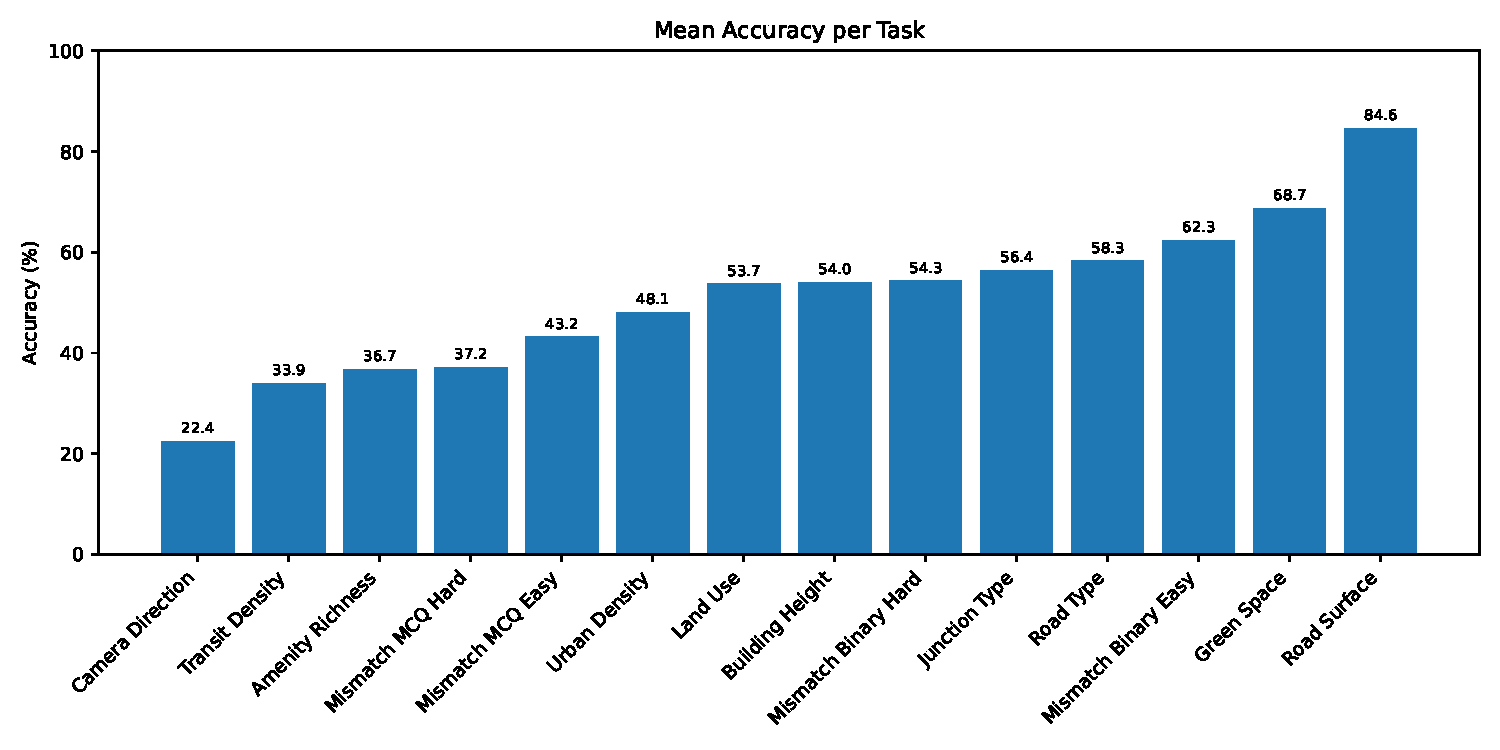
\includegraphics[width=\textwidth]{figures/mean_acc_per_task.pdf}
\caption{Mean accuracy across all four models per task, sorted ascending.
Tasks in the lower half represent open challenges for all current open-weights
VLMs on the EarthMLLMEval benchmark.}
\label{fig:mean_acc}
\end{figure}

% =====================================================================
\section{Benchmark Design Notes \& Evaluation Caveats}
% =====================================================================

\begin{itemize}[itemsep=4pt]

  \item \textbf{Answer-letter frequency imbalance.}
        Letters A and B appear as correct answers $\sim$29.3\% and
        29.6\% of the time respectively; C and D appear $\sim$20.2\%
        and 20.9\%. A model that always predicts B scores $\sim$29.6\%
        — just 10 points below Llama-3.2-Vision's 39.39\%. This
        imbalance is a known benchmark artefact (see dataset
        limitations).

  \item \textbf{F1 label-set bug (fixed, re-run pending).}
        The \texttt{mismatch\_binary} tasks have only 2 options (A/B)
        but were scored against the full 4-class \{A,B,C,D\} space.
        This artificially deflates F1 and AUC for those tasks by
        treating C and D as perpetually missed classes. Accuracy is
        unaffected. All F1 and AUC values in this report should be
        treated as preliminary. \textbf{F1 and AUC are therefore
        excluded from all primary figures and tables in this report.}

\end{itemize}

\begin{warnbox}[Re-run checklist]
Before citing any metric from this report in a paper, re-run the
evaluation with the fixed pipeline and verify:
(1) mismatch binary accuracy changes;
(2) F1 and AUC values stabilise with the correct label-set;
(3) MCQ accuracy improves with labeled composites.
Only \textbf{accuracy on non-mismatch tasks} is fully reliable in the
current results.
\end{warnbox}

% =====================================================================
\section{Conclusion}
% =====================================================================

This evaluation demonstrates that current open-weights VLMs at the 7--12B
parameter scale can solve visually clear urban recognition tasks at high
accuracy ($>$85\%) but consistently fail on tasks requiring cross-view
spatial grounding and geometric reasoning. The performance gap between the
best (PC-base, 62.86\%) and weakest added/base result (Qwen3.5-4B base, 35.48\%)
is 27.38 points — significant, but all models share the same failure modes.

\paragraph{Key conclusions.}
\begin{itemize}[itemsep=3pt]
  \item \textbf{Road surface and green space} are effectively solved
        by current VLMs; they add little discriminative value as future
        benchmark targets.
  \item \textbf{Mismatch binary hard} has a surprising 43-point range
        (Llama 44.18\% vs.\ Pixtral 87.17\%), suggesting this task
        may expose architectural differences between models better
        than any other.
  \item \textbf{Camera direction and mismatch MCQ hard} are genuinely
        unsolved. Near-random performance across all models indicates
        not just low accuracy but a complete absence of a reliable
        internal signal for these abilities.
  \item \textbf{Transit density and amenity richness} suffer from
        what appears to be fine-grained counting failure — models
        cannot reliably distinguish ``1--2 stops'' from ``3--5 stops''
        at the spatial scale of satellite imagery.
  \item \textbf{Non-standard camera angles} (along/cross) cause
        10--35 pp accuracy drops across all models, confirming that
        view-direction-aware reasoning is a critical missing capability.
  \item \textbf{Land-use context} matters: all models perform worst
        on open-space zones and best on mixed/residential contexts.
  \item \textbf{Generalisation to unseen cities is strong} ($\leq$3 pp drop),
        indicating that these tasks probe general visual reasoning
        rather than city-specific knowledge.
\end{itemize}

\paragraph{Future directions.}
Re-running with the fixed pipeline will provide clean accuracy, F1 and AUC
numbers for mismatch tasks. Beyond that, the benchmark points to four open
research directions: geometry-aware cross-view alignment, spatially grounded
semantic counting, direction-aware scene representation, and
camera-angle-robust feature extraction — none of which are adequately
handled by current pretraining objectives.

\end{document}
